\documentclass[assignment04_Solutions]{subfiles}

%\IfSubStr{\jobname}{\detokenize{Solutions}}{\toggletrue{solutions}}{\toggletrue{solutions}}

\IfSubStr{\jobname}{\detokenize{Solutions}}{\toggletrue{solutions}}{\togglefalse{solutions}}

\fancypagestyle{firstpage}

{\rhead{Assignment 4 \linebreak \textit{Version: \today}}}

\title{Assignment 4: Logistic Regression and Gradient Descent}
\author{Machine Learning}
\date{Fall 2021}

\begin{document}

\maketitle
\thispagestyle{firstpage}


\begin{learningobjectives}
\bi
\item Learn about the logistic regression algorithm.
\item Learn about gradient descent for optimization.
\item Contemplate an application of machine learning for home loans.
\ei
\end{learningobjectives}

\begin{priorknowledge}
\bi
\item Supervised learning problem framing.
\item Calculating gradients.
\item Log loss.

\ei
\end{priorknowledge}
\vspace{1em}

%
%\begin{recall}[Supervised Learning Problem Setup]
%We are given a training set, $(\mlvec{x_1}, y_1), (\mlvec{x}_2, y_2), \ldots, (\mlvec{x}_n, y_n)$ where each $\mlvec{x_i}$ represents an element of an input space (e.g., a d-dimensional feature vector) and each $y_i$ represents an element of an output space (e.g., a scalar target value).  Our goal is to determine a function $\hat{f}$ that maps from the input space to the output space.
%
%We assume there is a loss function, $\ell$, that determines the amount of loss that a particular prediction $\hat{y}_i$ incurs due to a mismatch with the actual output $y_i$.  The best possible model, $\hat{f}^\star$, is the one that minimizes these losses over the training set.  This notion can be expressed with the following equation.
%\begin{align}
%\hat{f}^\star &= \argmin_{\hat{f}} \sum_{i=1}^n \ell \left ( \hat{f}(\mlvec{x_i}), y_i \right )
%\end{align} 
%\end{recall}

\section{Logistic Regression (top-down)}

In the last part of the \href{https://colab.research.google.com/drive/1AOUbSKhEvoSTzu_UNm-kq1SBrmmXPHVl?usp=sharing}{notebook that you started in class}, you saw a quick implementation of logistic regression to classify if a person was looking to the left or to the right. 

In this assignment we will formalize the binary classification problem and dig the theory behind \emph{logistic regression}.  You will also see that the logistic regression algorithm is a very natural extension of linear regression.  Our plan for getting there is going to be pretty similar to what we did for linear regression.
\bi
\item Build some mathematical foundations
\item Introduce logistic regression from a top-down perspective
\item Learn about logistic regression from a bottom-up perspective
\ei



\begin{recall}
In the last assignment, you were introduced to the idea of binary classification, which based on some input $\mlvec{x}$ has a corresponding output $y$ that is $y= 0$ or $y= 1$. In logistic regression, this model, $\hat{f}$, instead of spitting out either 0 or 1, outputs a confidence that the input $\mlvec{x}$ has an output $y= 1$.  In other words, rather than giving us its best guess (0 or 1), the classifier indicates to us its degree of certainty regarding its prediction as a probability.

We also explored three possible loss functions for a model that outputs a probability $p$ when supplied with an input $\mlvec{x}$ (i.e., $\hat{f}(\mlvec{x})=p$). The loss function is used to quantify how bad a prediction $p$ is given the actual output $y$ (for binary classification the output is either $0$ or $1$).

\be
\item \textbf{0-1 loss:} This is an all-or-nothing approach. If the prediction is correct, the loss is zero; if the prediction is incorrect, the loss is 1. This does not take into account the level certainty expressed by the probability (the model gets the same loss if $y = 1$ and it predicted $p = 0.51$ or $p = 1$).
\item \textbf{squared loss:}  For squared loss we compute the difference between the outcome and $p$ and square it to arrive at the loss.  For example, if $y = 1$ and the model predicts $p = 0.51$, the loss is $(1 - 0.51)^2$.  If instead $y = 0$, the loss is $(0 - 0.51)^2$.
\item \textbf{log loss:} The log loss also penalizes based on the difference between the outcome and $p$, using the formula below.
\begin{align}
 logloss = -\frac{1}{N}\sum_{i=1}^n ( (y_i) \ln (p_i) + (1-y_i) \ln (1 - p_i) )\label{eq:loglosseq}
\end{align}
Since $y_i$ is always 0 or 1, we will essentially switch between the two chunks of this equation based on the true value of $y_i$. As the predicted probability, $p_i$ (which is constrained between 0 an 1) gets farther from $y_i$, the log-loss value increases.

\ee



\end{recall}





Now that you have refreshed on how probabilities can be used as a way of quantifying confidence in predictions, you are ready to learn about the logistic regression algorithm.

As always, we assume we are given a training set of inputs and outputs.  As in linear regression we will assume that each of our inputs is a $d$-dimensional vector $\mathbf{x_i}$ and since we are dealing with binary classification, the outputs, $y_i$, will be binary numbers (indicating whether the input belongs to class 0 or 1).  Our hypothesis functions, $\hat{f}$, output the probability that a given input has an output of 1.  What's cool is that we can borrow a lot of what we did in the last couple of assignments when we learned about linear regression.  In fact, all we're going to do in order to make sure that the output of $\hat{f}$ is between 0 and 1 is pass $\mlvec{w}^\top \mlvec{x}$ through a function that ``squashes'' its input so that it outputs a value between 0 and 1.  This idea is shown graphically in Figure~\ref{fig:graphicaldataflow}.

\begin{marginfigure}
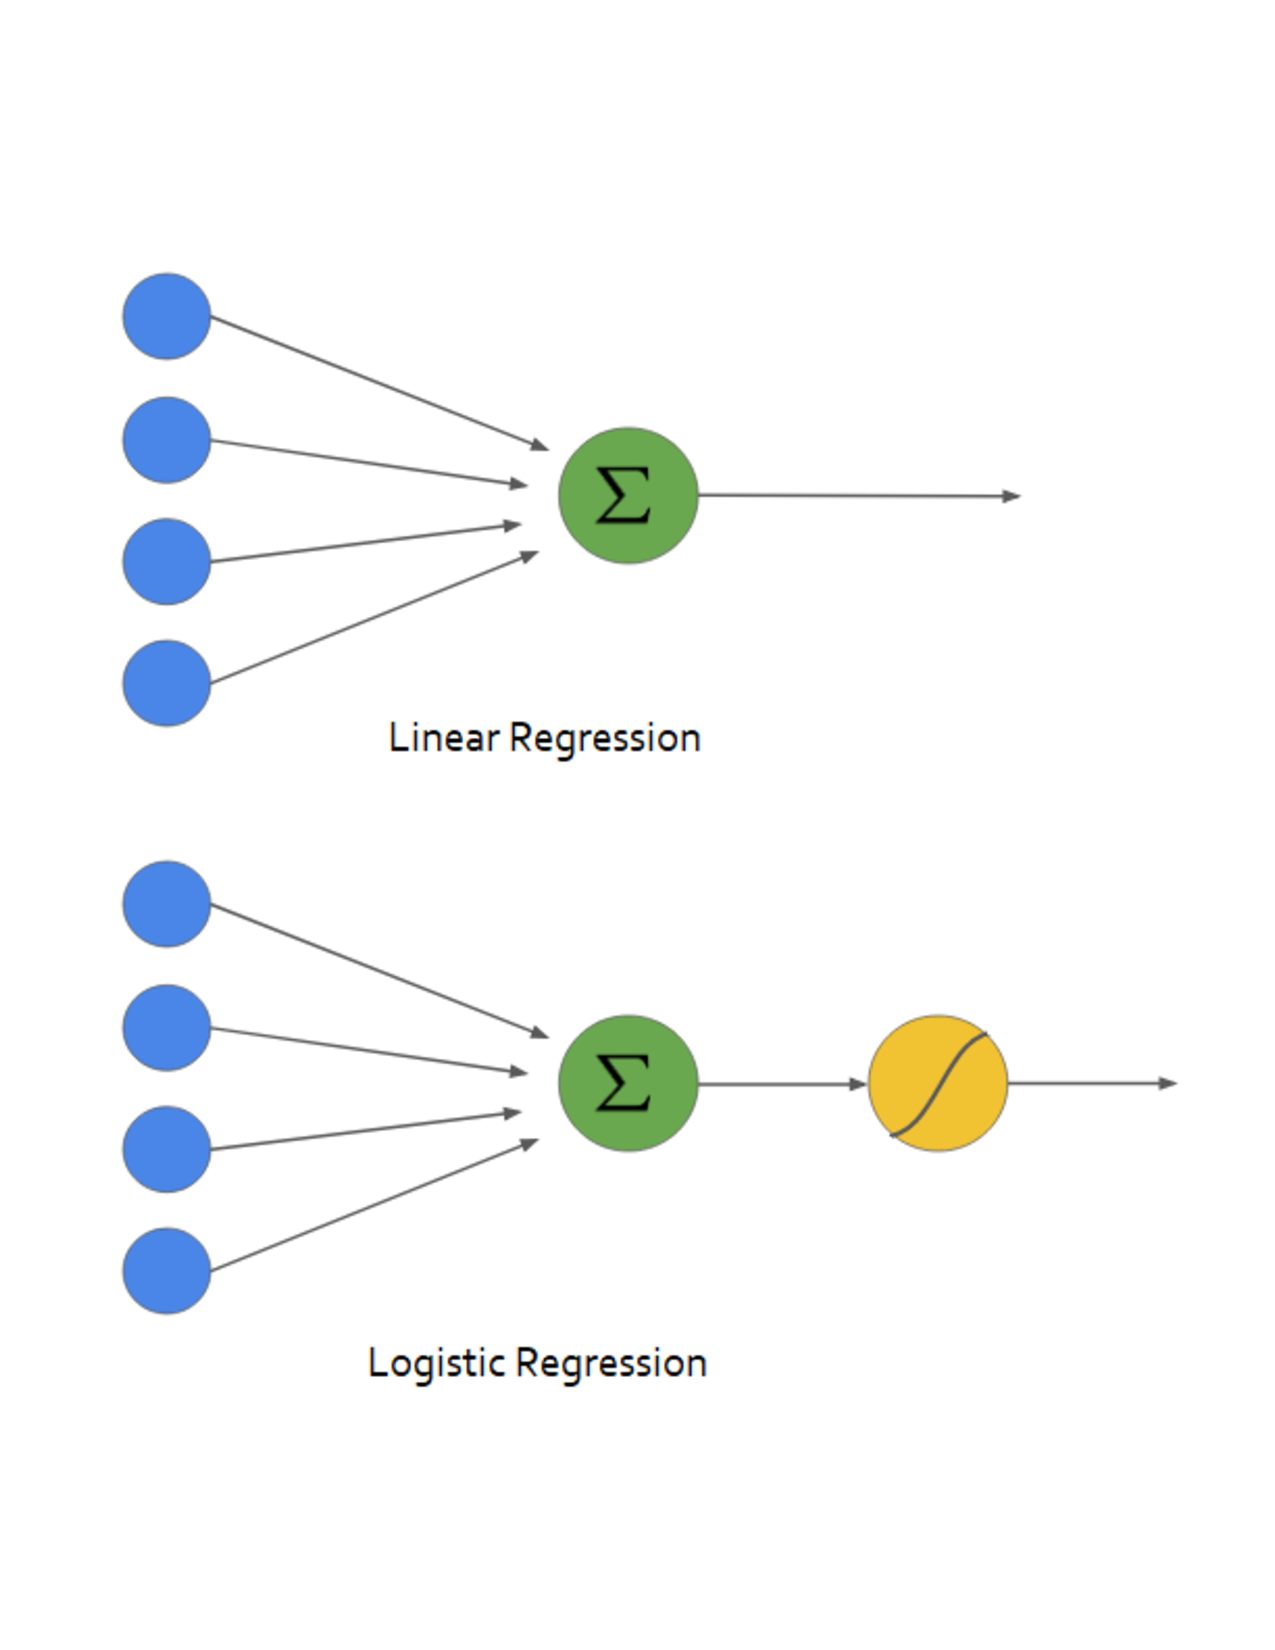
\includegraphics[height=2in]{figures/linearandlogistic}
\caption{Graphical representation of both linear and logistic regression.  The key difference is the application of the squashing function shown in yellow.  \href{https://towardsdatascience.com/building-a-logistic-regression-in-python-301d27367c24}{Original source}.}\label{fig:graphicaldataflow}

\end{marginfigure}
To make this intuition concrete, we define each $\hat{f}$ as having the following form (note: this equation looks daunting. We have some tips for interpreting it below).

\begin{align}
\hat{f}(\mathbf{x}) &= \mbox{probability that output, $y$, is 1} \nonumber \\
&=\frac{1}{1 + e^{-\mlvec{w}^\top \mathbf{x}}} \label{eq:logistichypothesis}
\end{align}

Here are a few things to notice about this equation:
\be
\item The weight vector that we saw in linear regression, $\mlvec{w}$, has made a comeback. We are using the dot product between $\mlvec{x}$ and $\mlvec{w}$ (which creates a weighted sum of the $x_i$'s), just as we did in linear regression!
\item As indicated in Figure~\ref{fig:graphicaldataflow}, the dot product $\mlvec{w}^\top \mlvec{x}$ has been passed through a squashing function known as the \href{https://en.wikipedia.org/wiki/Sigmoid_function}{sigmoid function}.  The graph of $\sigma(u) = \frac{1}{1+e^{-u}}$ is shown in Figure~\ref{fig:sigmoid}.  $\sigma( \mlvec{w}^\top \mlvec{x})$ is exactly what we have in Equation~\ref{eq:logistichypothesis}. 

\begin{marginfigure}
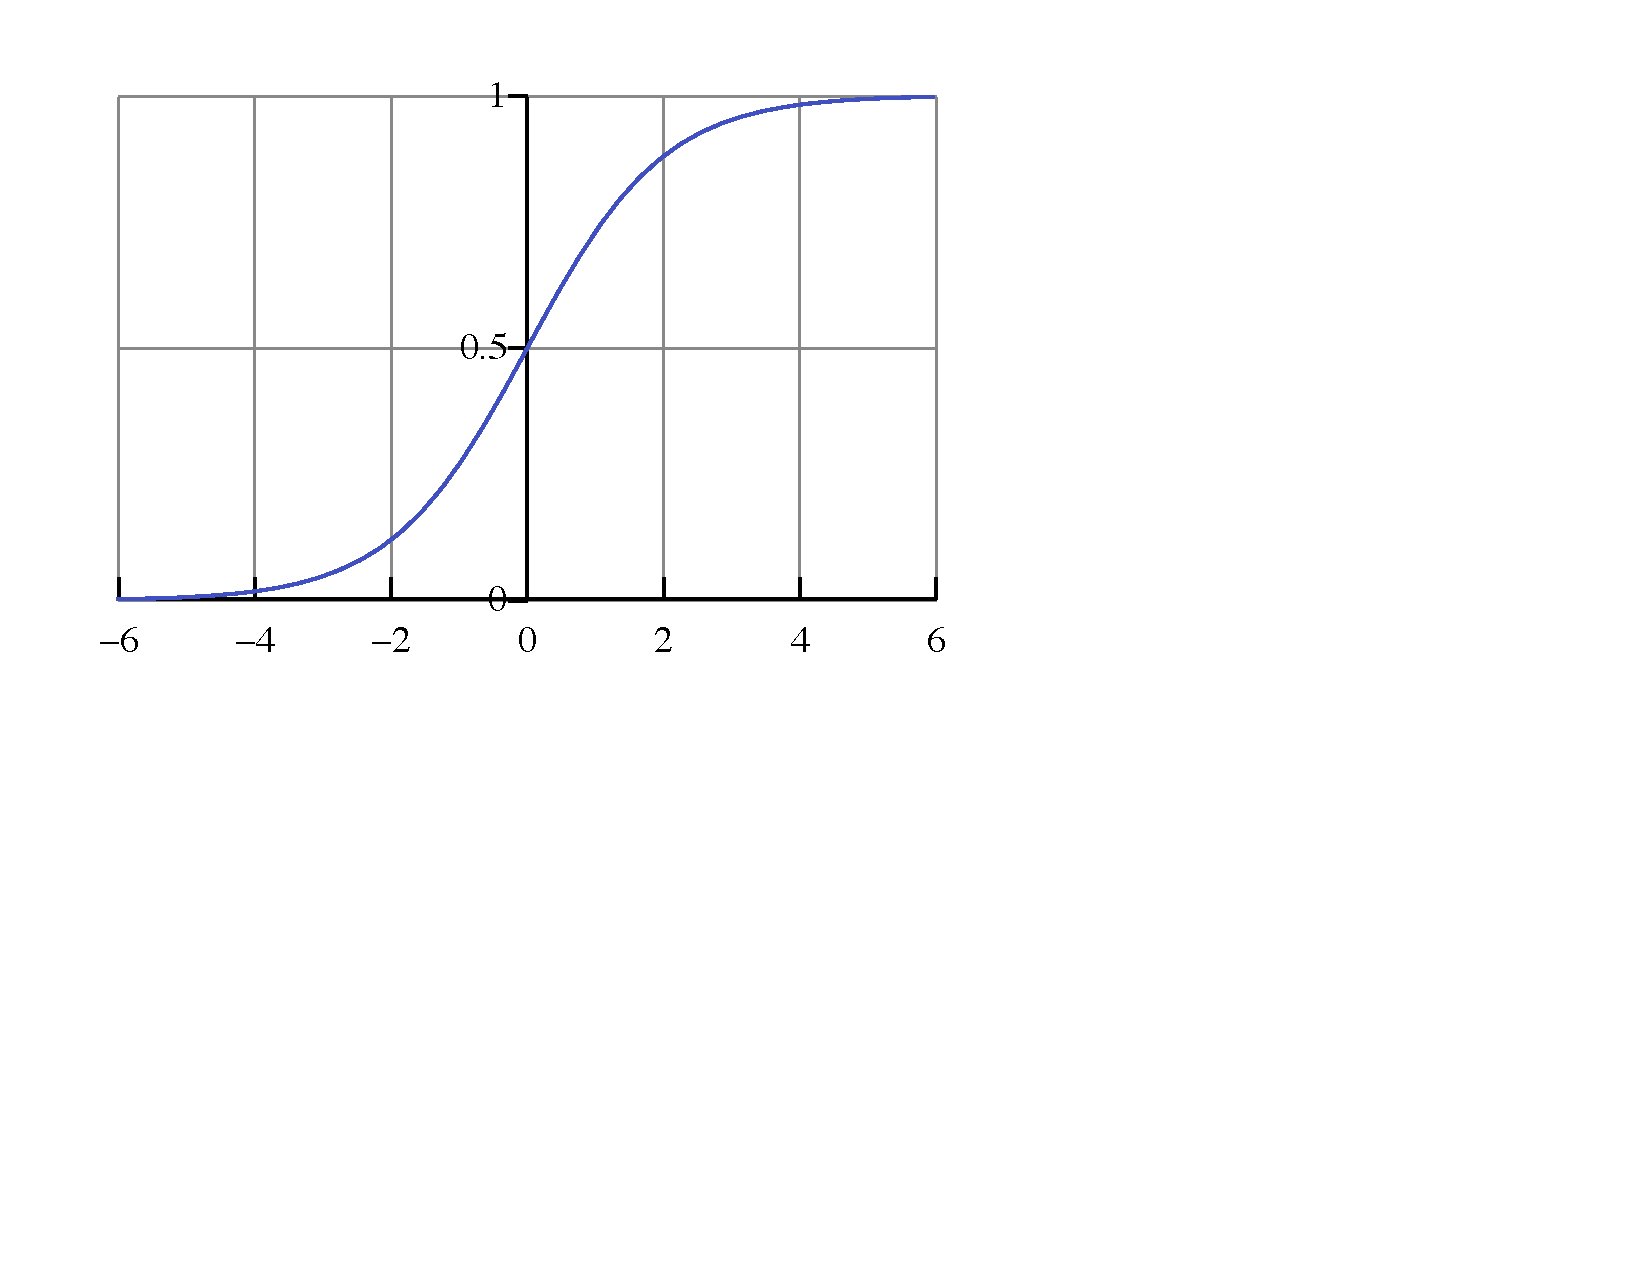
\includegraphics[width=\linewidth]{figures/Logistic-curve}
\caption{a graph of the sigmoid function $\frac{1}{1+e^{-x}}$.}\label{fig:sigmoid}
\end{marginfigure}
\ee

%\subsection{Motivating Example: Sensor Networks}

%\begin{notice}
%Pretty much every writeup of logistic regression contains a simple two-independent variable example.  Usually these examples involve things like predicting who would be approved for a credit card or who will be admitted to a college.  We are going to do something a little messier and bit different.  If you want the admission to college example, you can read about it in \href{https://towardsdatascience.com/building-a-logistic-regression-in-python-301d27367c24}{Building a Logistic Regression in Python}.
%\end{notice}

%\begin{externalresources}[(60 minutes)]
%Switch on over to the \href{https://colab.research.google.com/github/mlfa19/assignments/blob/master/Module\%201/03/Assignment_03_Companion.ipynb}{Assignment 3 Companion Notebook} for a presentation of the motivating example.
%\end{externalresources}

\section{Deriving the Logistic Regression Learning Rule}
%Let's summarize what we've done thus far in this assignment.

%\bi
%\item We motivated the binary classification problem.
%\item We presented a particular useful loss function (log loss).
%\item We met the logistic regression model and tried it out on a real dataset.
%\ei

Now we will formalize the logistic regression problem and derive a learning rule to solve it (i.e., compute the optimal weights). The formalization of logistic regression will combine Equation~\ref{eq:logistichypothesis} with the selection of $\ell$ to be log loss (Equation~\ref{eq:loglosseq}).  This choice of $\ell$ results in the following objective function.

\begin{align}
\mlvec{w}^\star &= \argmin_{\mlvec{w}} \sum_{i=1}^n \left ( - y_i \ln \sigma(\mlvec{w}^\top \mlvec{x_i}) - (1-y_i) \ln (1 - \sigma(\mlvec{w}^\top \mlvec{x_i}) ) \right) \\
&= \argmin_{\mlvec{w}} \sum_{i=1}^n \left (  - y_i \ln \left ( \frac{1}{1+e^{-\mlvec{w}^\top \mlvec{x_i}}} \right) - (1-y_i) \ln  \left (1 - \frac{1}{1+e^{-\mlvec{w}^\top \mlvec{x_i}}} \right ) \right) &\mbox{expanded out if you prefer this form} \label{eq:objective}
\end{align}

While this looks a bit intense, since $y_i$ is either 0 or 1, the multiplication of the expressions in the summation by either $y_i$ or $1-y_i$ are essentially acting like a switch---depending on the value of $y_i$ we either get one term or the other.  Our typical recipe for finding $\mlvec{w}^\star$ has been to take the gradient of the expression inside the $\argmin$, set it to $0$, and solve for $\mlvec{w}^\star$ (which will be a critical point and hopefully a minimum).  The last two steps will be a bit different for reasons that will become clear soon, but we will need to find the gradient.  We will focus on finding the gradient in the next couple of parts.

\subsection{Useful Properties of the Sigmoid Function}

Looking at Equation~\ref{eq:objective} it looks really, really hairy!  We see that in order to compute the gradient we will have to compute the gradient of $\mathbf{x}^\top \mlvec{w}$ with respect to $\mlvec{w}$ (we just wrapped our minds around this last assignment).  Additionally, we will have to take into account how the application of the sigmoid function and the log function changes this gradient.  In this section we'll learn some properties for manipulating the sigmoid function and computing its derivative.

\begin{exercise}[(60 minutes)]
The sigmoid function, $\sigma$, is defined as

\begin{align}
\sigma(x) &= \frac{1}{1+e^{-x}} \enspace .
\end{align}

\bes
\item Show that $\sigma(-x) = 1 - \sigma(x)$.
\begin{boxedsolution}
\begin{align}
\sigma(-x) &= \frac{1}{1+e^{x}} \\
&= \frac{e^{-x}}{e^{-x} + 1}~~\mbox{multiply by top and bottom by $e^{-x}$} \\
 \sigma(-x)  - 1&= \ \frac{e^{-x}}{e^{-x} + 1} - \frac{1 + e^{-x}}{1 + e^{-x}} ~~\mbox{subtract $-1$ on both sides} \\
 &= \frac{-1}{1+e^{-x}} \\
 &= -\sigma(x) \\
 \sigma(-x) &= 1 - \sigma(x)
\end{align}
\end{boxedsolution}
\item Show that the derivative of the logistic function $\frac{d}{dx} \sigma(x) = \sigma(x) (1 - \sigma(x))$

\begin{boxedsolution}
Two solutions for the price of 1!

Solution 1:
\begin{align}
\frac{d}{dx} \sigma(x)  &= e^{-x} \sigma(x)^2 &\mbox{\href{https://www.math.hmc.edu/calculus/tutorials/quotient_rule/}{apply quotient rule}} \\
&= \sigma(x) \left ( \frac{e^{-x}}{1 + e^{-x}} \right) &\mbox{expand out one of the $\sigma(x)$'s}\\
&= \sigma(x) \left ( \frac{1}{e^{x} + 1} \right) & \mbox{multiply top and bottom by $e^{x}$}\\
&=  \sigma(x) (  \sigma(-x)) &\mbox{substitute for $\sigma(-x)$} \\
&=  \sigma(x) (1 -  \sigma(x) ) &\mbox{apply $\sigma(-x)=1-\sigma(x)$}
\end{align}

Solution 2:
\begin{align}
\frac{d}{dx} \sigma(x)  &=\frac{e^{-x}}{(1+e^{-x} )^2} & \mbox{\href{https://www.math.hmc.edu/calculus/tutorials/quotient_rule/}{apply quotient rule}} \\
&= \frac{e^{-x}}{1+2e^{-x} + e^{-2x}} & \mbox{expand the bottom}\\
&= \frac{1}{e^{x}+2 + e^{-x}} & \mbox{multiply top and bottom by $e^{x}$}\\
&= \frac{1}{(1+e^{x})(1+e^{-x})} & \mbox{factor} \\
&= \sigma(x)\sigma(-x) & \mbox{decompose using definition of $\sigma(x)$}\\
&= \sigma(x)(1-\sigma(x)) &\mbox{apply $\sigma(-x)=1-\sigma(x)$}
\end{align}

\end{boxedsolution}
%
%\item \textbf{considering making this optional or just deleting} The log odds of an event occurring is defined as 
%\begin{align}
%\ln \left ( \frac{p(\mbox{event occurs})}{p(\mbox{event does not occur})} \right) = \ln \left ( \frac{p(\mbox{event occurs})}{1 - p(\mbox{event does occur})} \right) \enspace .
%\end{align}
%
%If we assume that $p(\mbox{event occurs}) = \sigma(x)$, show that the log odds of the event occurring is equal to $x$.
%
%\begin{boxedsolution}
%\begin{align}
%\ln \left ( \frac{p(\mbox{event occurs})}{p(\mbox{event does not occur})} \right)  &= \ln \left ( \frac{\sigma(x)}{1 - \sigma(x)} \right ) \\
%&= \ln \left ( \frac{\sigma(x)}{\sigma(-x)} \right ) \\
%&= \ln \left ( \frac{1 + e^x}{1+e^{-x}} \right) \\
%&= \ln \left ( e^x \frac{1 + e^x}{e^{x}(1+e^{-x})} \right) \\
%&= x + \ln \left ( \frac{1+e^x}{e^{x} + 1} \right) \\
%&= x
%\end{align}
%\end{boxedsolution}

\ees

\end{exercise}

\subsection{Chain Rule for Gradients}
We now know how to take derivatives of each of the major pieces of Equation~\ref{eq:objective}.  What we need is a way to put these derivatives together.  You probably remember that in the case of single variable calculus you have just such a tool.  This tool is known as the chain rule.  The chain rule tells us how to compute the derivative of the composition of two single variable functions $f$ and $g$.  

\begin{align}
h(x)&= g(f(x))&\mbox{h(x) is the composition of $f$ with $g$} \nonumber \\
h'(x) &= g'(f(x))f'(x)&\mbox{this is the chain rule!}
\end{align}

Suppose that instead of the input being a scalar $x$, the input is now a vector, $\mlvec{w}$.  In this case $h$ takes a vector input and returns a scalar, $f$ takes a vector input and returns a scalar, and $g$ takes a scalar input and returns a scalar.

\begin{align}
h(\mlvec{w}) &= g(f(\mlvec{w}))&\mbox{h($\mlvec{w}$) is the composition of $f$ with $g$} \nonumber \\
\nabla h(\mlvec{w}) &= g'(f(\mlvec{w})) \nabla f(\mlvec{w}) & \mbox{this is the multivariable chain rule}
\end{align}

\begin{exercise}[(60 minutes)]
\bes
\item Suppose $h(x) = \sin(x^2)$, compute $h'(x)$ (x is a scalar so you can apply the single-variable chain rule).

\begin{boxedsolution}

Applying the chain rule gives
\begin{align}
h'(x) &= cos(x^2) 2x \enspace .
\end{align}
\end{boxedsolution}

\item Define $h(\mlvec{v}) = (\mlvec{c}^\top \mlvec{v})^2$.  Compute $\nabla_{\mlvec{v}} h(\mlvec{v})$ (the gradient of the function with respect to $\mlvec{v}$).

\begin{boxedsolution}
We can see that $h(\mlvec{v}) = g(f(\mlvec{v}))$ with $g(x) = x^2$ and $f(\mlvec{v}) = \mlvec{c}^\top \mlvec{v}$ The gradient can now easily be found by applying the chain rule.
\begin{align}
\nabla h(\mlvec{v}) &= 2(\mlvec{c}^\top \mlvec{v}) \mlvec{c}
\end{align}
\end{boxedsolution}

\item Compute the gradient of the expression from Equation~\ref{eq:objective} (reproduced below for your convenience).

\begin{align}
 \sum_{i=1}^n -y_i \ln \sigma( \mlvec{w}^\top \mlvec{x_i}) - (1-y_i) \ln  \left (1 - \sigma( \mlvec{w}^\top \mlvec{x_i}) \right ) \enspace .
\end{align}

You can either use the chain rule and the identities you learned about sigmoid, or expand everything out and work from that.

\begin{boxedsolution}
Applying the chain rule gives us

\begin{align}
 \sum_{i=1}^n -y_i \frac{\nabla \sigma( \mlvec{w}^\top \mlvec{x_i})}{\sigma( \mlvec{w}^\top \mlvec{x_i})} - (1-y_i) \frac{- \nabla \sigma( \mlvec{w}^\top \mlvec{x_i})}{1 - \sigma( \mlvec{w}^\top \mlvec{x_i})}  \enspace .
\end{align}

Applying the chain rule again gives us
\begin{align}
& \sum_{i=1}^n -y_i \frac{\sigma( \mlvec{w}^\top \mlvec{x_i})(1-\sigma( \mlvec{w}^\top \mlvec{x_i}))\nabla \mlvec{w}^\top \mlvec{x_i}}{\sigma( \mlvec{w}^\top \mlvec{x_i})} - (1-y_i) \frac{- \sigma( \mlvec{w}^\top \mlvec{x_i})(1-\sigma( \mlvec{w}^\top \mlvec{x_i}))\nabla \mlvec{w}^\top \mlvec{x_i}}{1 - \sigma( \mlvec{w}^\top \mlvec{x_i})} \nonumber \\
 &= \sum_{i=1}^n -y_i (1-\sigma( \mlvec{w}^\top \mlvec{x_i}))\mlvec{x_i} + (1-y_i)  \sigma( \mlvec{w}^\top \mlvec{x_i})) \mlvec{x_i} 
 \end{align}
 
You could certainly stop here, but if you plug in $y=0$ and $y=1$ you'll find that the expression can be further simplified to:
 
 \begin{align}
\sum_{i=1}^n  -(y_i - \sigma(\mlvec{w}^\top \mlvec{x_i})) \mlvec{x_i} \nonumber
 \end{align}


\end{boxedsolution}

\ees
\end{exercise}


\subsection{Gradient Descent for Optimization}
If we were to follow our derivation of linear regression we would set our expression for the gradient to 0 and solve for $\mlvec{w}$.  It turns out this equation will be difficult to solve due to the $\sigma$ function.  Instead, we can use an iterative approach where we start with some initial value for $\mlvec{w}$ (we'll call the initial value $\mlvec{w^0}$, where the superscript corresponds to the iteration number) and iteratively adjust it by moving down the gradient (the gradient represents the direction of fastest increase for our function, therefore, moving along the negative gradient is the direction where the loss is decreasing the fastest).

\vspace{1em}
\begin{externalresources}[(45 minutes)]
There are tons of great resources that explain gradient descent with both math and compelling visuals.
\bi
\item Recommended: \href{https://www.youtube.com/watch?v=IHZwWFHWa-w}{Gradient descent, how neural networks learn | Deep learning, chapter 2} (start at 5:20)
\item \href{https://medium.com/@viveksingh.heritage/an-introduction-to-gradient-descent-54775b55ba4f}{An Introduction to Gradient Descent}
\item \href{https://en.wikipedia.org/wiki/Gradient_descent}{The Wikipedia page on Gradient Descent}
\item \href{https://www.youtube.com/watch?v=fPSPdTjINi0}{Ahmet Sacan's video on gradient descent} (this one has some extra stuff, but it's pretty clearly explained).
\item There are quite a few resources out there, do you have some suggestions? (suggest so on Discord)
\ei 
\end{externalresources}

\begin{exercise}[(10 minutes)]
To test your understanding of these resources, here are a few diagnostic questions.
\bes
\item When minimizing a function with gradient descent, which direction should you step along in order to arrive at the next value for your parameters?
\begin{boxedsolution}
The negative gradient (since we are minimizing)
\end{boxedsolution}

\item What is the learning rate and what role does it serve in gradient descent?
\begin{boxedsolution}
The learning rate controls the size of the step that you take along the negative gradient.
\end{boxedsolution}

\item How do you know when an optimization performed using gradient descent has converged?
\begin{boxedsolution}
There are a few options.  One popular one is to check if the objective function is changing only only a minimal amount each iteration, the algorithm has converged.  You could also look at the magnitude of the gradient (which tells us the slope) to see if it is really small.
\end{boxedsolution}

\item True or false: provided you tune the learning rate properly, gradient descent guarantees that you will find the global minimum of a function.
\begin{boxedsolution}
False, the best gradient descent can do, in general, is converge to a local minimum.  If you know that the function you are optimizing has only one minimum, then this would also be the global minimum (this is the case for both linear and logistic regression).
\end{boxedsolution}
\ees
\end{exercise}

If we take the logic of gradient descent and apply it to the logistic regression problem, we arrive at the following learning rule.  Given some initial weights $\mlvec{w^0}$, and a learning rate $\eta$, we can iteratively update our weights using the formula below.

\begin{align}
\mlvec{w^{n+1}} &= \mlvec{w^n} - \eta \sum_{i=1}^n  -(y_i - \sigma(\mlvec{w}^\top \mlvec{x_i})) \mlvec{x_i} ~~~\mbox{applying the result from exercise 2} \\
&=  \mlvec{w^n} + \eta \sum_{i=1}^n  (y_i - \sigma(\mlvec{w}^\top \mlvec{x_i})) \mlvec{x_i}  ~~~\mbox{distribute the negative}
\end{align}

This beautiful equation turns out to be the recipe for logistic regression. \\

\begin{notice}
We won't be assigning a full implementation of logistic regression from scratch. In future assignments, we will spend more time applying logistic regression and gradient descent. 

If it's helpful for your learning to see a worked example with code now (to help the math make sense), you can optionally check out this \href{https://towardsdatascience.com/building-a-logistic-regression-in-python-301d27367c24}{example of binary classification for admission to college}, noting that some of the math notation is slightly different than ours. 

You are also welcome to implement logistic regression using gradient descent if it's helpful for your learning and/or if you already have significant experience with machine learning and want a challenge. This is completely optional, and we assume that most of you will not choose to do this. If you do decide to implement logistic regression using gradient descent, you will need to search for a good learning rate or you may consider implementing some \href{https://towardsdatascience.com/gradient-descent-algorithms-and-adaptive-learning-rate-adjustment-methods-79c701b086be}{strategies for automatically tuning the learning rate}.


\end{notice}





\section{Touchpoint to context, impact, and ethics}

As we mentioned in the introduction to the course, we'll be exploring machine learning from three different perspectives: the theory, the implementation, and the context, impact, and ethics. 

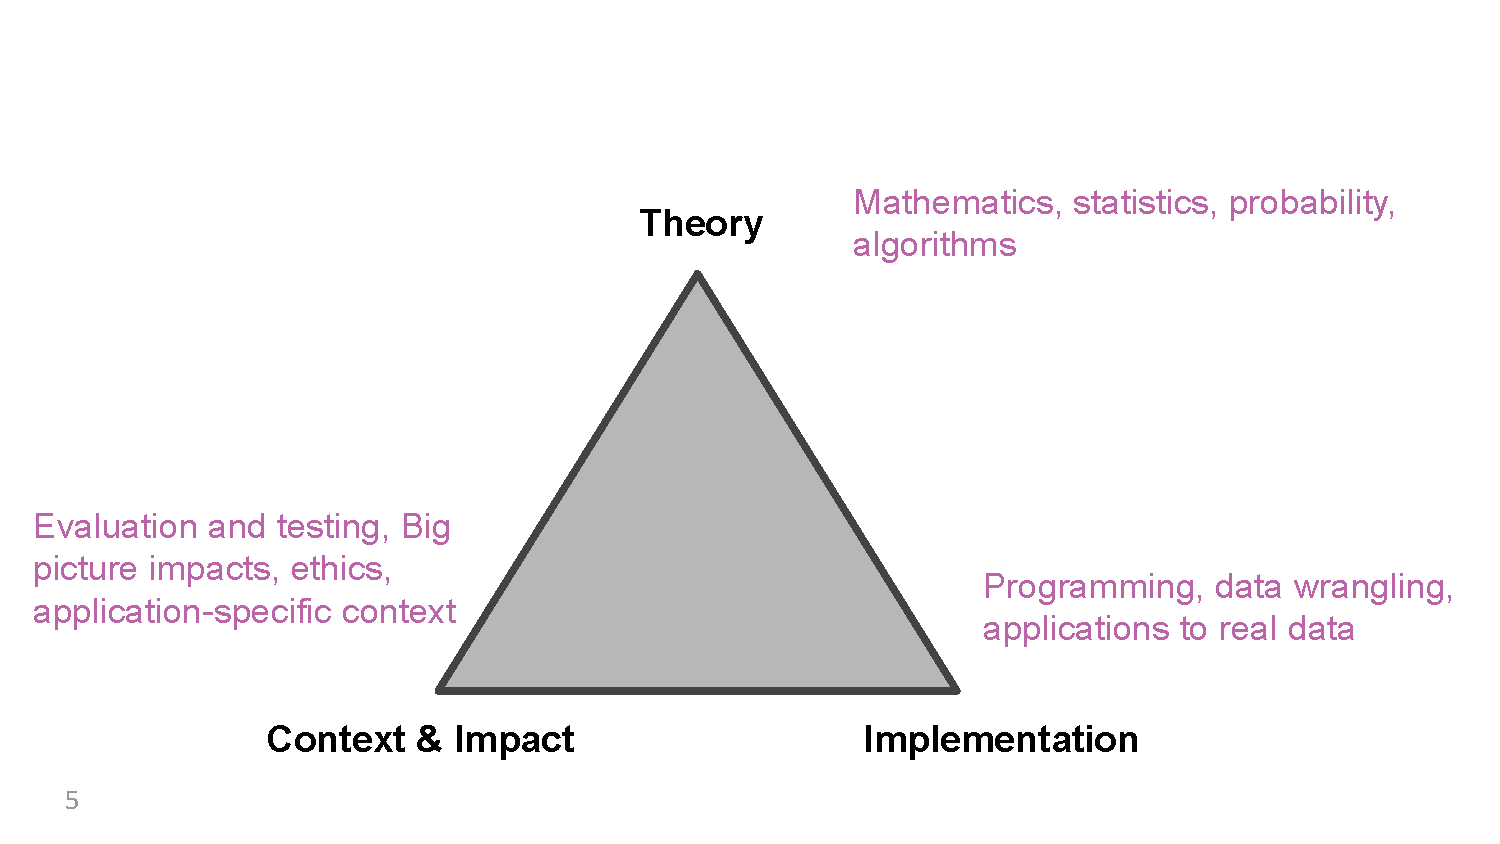
\includegraphics[height=2in]{figures/ternaryTIE}

Lately, we've been diving deeply into the mathematical theory with some touch points in implementation and context. Here, we want to take a moment to zoom out (with a lowercase z), and think about how algorithms interact with society, individuals, and institutions. 

%\todo[inline]{one option, carrie is only 45 min into it and felt like it started strong but lost the plot, not sure I have another 1.5 hours to watch another}
%We are going to take a virtual field trip to a leading conference on this topic! In normal times it would be challenging and expensive for us to bring the entire class to this conference, but thanks to the pandemic we can easily share one of the talks from the Conference on Fairness, Accountability, and Transparency with you. 
%
%\begin{exercise}
%Please watch \href{https://www.youtube.com/watch?v=rSOZhv4bqQU&list=PLXA0IWa3BpHnYVwSLuvv1Jv1U1Pyhcymt&index=8}{this talk} and take notes. 
%\end{exercise}
%
%\todo[inline]{Or, option 2-- Carrie likes this one better, and it's closer to an hour. I'm not sure it captures the magic Sam was looking for.}

Machine learning governs how people can access wealth-building tools, like loans and mortgages.
Please read \href{https://www.nytimes.com/2020/09/18/business/digital-mortgages.html}{this article on algorithms preventing bias in home loans.} Then watch \href{https://www.ted.com/talks/shivani_siroya_a_smart_loan_for_people_with_no_credit_history_yet/up-next?language=en}{this TED talk} about a way to build credit history.
\begin{exercise}
Consider the following questions.
\begin{enumerate}
\item Would you consider the NY Times story objective? What about the TED talk?
\begin{boxedsolution}
The NY Times story seems very one-sided. Although the examples of benefits to algorithms are good, the reporter basically talked to people the company had vetted. What about unhappy users of the service? It's pretty poor reporting. Shivani's TED talk is compelling, but she's also an entrepreneur trying to get interest in her company.
\end{boxedsolution}

\item Consider the pros and cons of using Tala, Shivani's company. What are the users gaining? What are they giving up? Is what they give up different than what users of a credit report provide?

\item Here's \href{https://tala.co/data-ethics/}{Tala's Statement on Data Ethics}. How does it compare to the FAT-ML framework we looked at on Day 1?
\end{enumerate}
\end{exercise}


% carrie likes this talk because it highlights ways transparency isn't advantageous. Unlike some of the other talks, it's just negative examples of ML

%\todo[inline]{Need exercise here on what to watch from ACM FAccT 2021 Tutorials https://www.youtube.com/playlist?list=PLXA0IWa3BpHnYVwSLuvv1Jv1U1Pyhcymt}

%
%
%
%\section{Reading on TODO}
%TODO
%
%\section{Suggestions for Additional Challenge (NOTE: I'm on the fence about these.  What do you think?}
%
%We are asking folks for whom this is review to push themselves a bit farther.  Based on the first two assignments, we thought that we could help out with some suggestions of our own.  Please don't construe this as work that you have to do.  None of the course content will assume that you've done any of these additional activities.
%
%\begin{itemize}
%\item Implement logistic regression using gradient descent.  You will need to search for a good learning rate or you may consider implementing some \href{https://towardsdatascience.com/gradient-descent-algorithms-and-adaptive-learning-rate-adjustment-methods-79c701b086be}{strategies for automatically tuning the learning rate}.
%\item Some additional reading?
%\end{itemize}

%\companionnotebook{Assignment_03_Companion}


\end{document}
